\documentclass[14pt]{extarticle}

\usepackage[LGR]{fontenc}
\usepackage[main=greek,english]{babel}
\usepackage[utf8]{inputenc}
\usepackage[unicode]{hyperref}
\usepackage{titlepic}
\usepackage{graphicx}
\usepackage{listings}

\graphicspath{ {./img/} }

\usepackage{listings}
\usepackage{xcolor}

\hyphenpenalty=10000
\hbadness=10000

\definecolor{codegreen}{rgb}{0,0.6,0}
\definecolor{codegray}{rgb}{0.5,0.5,0.5}
\definecolor{codepurple}{rgb}{0.58,0,0.82}
\definecolor{backcolour}{rgb}{0.95,0.95,0.92}

\lstdefinestyle{mystyle}{
    backgroundcolor=\color{backcolour},   
    commentstyle=\color{codegreen},
    keywordstyle=\color{magenta},
    numberstyle=\tiny\color{codegray},
    stringstyle=\color{codepurple},
    basicstyle=\ttfamily\footnotesize,
    breakatwhitespace=false,         
    breaklines=true,                 
    captionpos=b,                    
    keepspaces=true,                 
    numbers=left,                    
    numbersep=5pt,                  
    showspaces=false,                
    showstringspaces=false,
    showtabs=false,                  
    tabsize=2
}

\lstset{frame=shadowbox, framexleftmargin=4mm, rulesepcolor=\color{black}, style=mystyle}

\title{\bfΕργασία Μεταγλωττιστών \\ Τμήμα Α2}
\titlepic{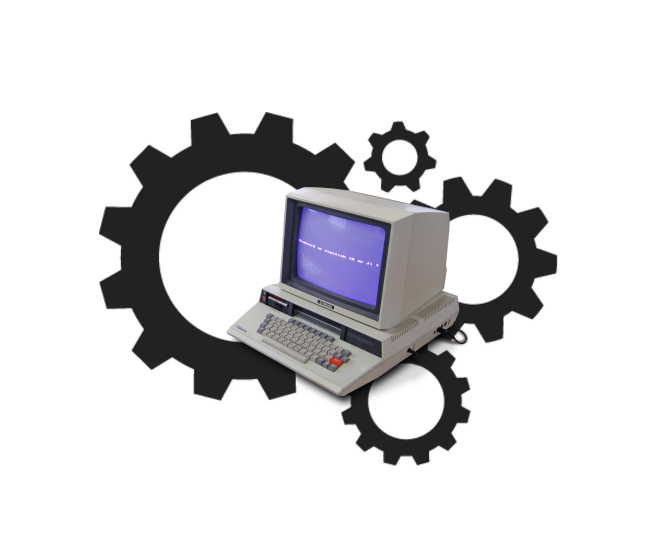
\includegraphics[scale=2.5]{computer.png}}
\author{
  \emph{Ομάδα 15}
}

\begin{document}

\begin{titlepage}
  \maketitle
  \begin{center}
    \large \emph{Ομάδα 15}
    \\
    Αναλυτικά τα μέλη:
\vspace{5mm}
  \begin{tabular}{r l}
    \\Διονύσης Νικολόπουλος & $AM: 18390126$
    \\Θανάσης Αναγνωστόπουλος & $AM: 18390043$
    \\Αριστείδης Αναγνωστόπουλος & $AM: 16124$
    \\Σπυρίδων Φλώρος & $AM: 141084$
  \end{tabular}
\vspace{5mm}
    \\
    Αναλυτικά οι ρόλοι:
    \\
\vspace{5mm}
  \begin{tabular}{r l}
    \small Γενικός Συντονιστής:   Διονύσης Νικολόπουλος
    \\
    \small Υπεύθυνος Τμήματος Εργασίας Α2: Διονύσης Νικολόπουλος
  \end{tabular}
  \\
\vspace*{\fill}
    \footnotesize{Η εργασία αυτή πραγματοποιήθηκε με χρήση \LaTeX}}
  \end{center}
\end{titlepage}
\tableofcontents


\section*{Διάγραμμα Ενιαίου Αυτόματου}
\smallΕδώ είναι το ενιαίο αυτόματο που σχεδιάσαμε με την βοήθεια του προγράμματος \textlatin{JFLAP}.
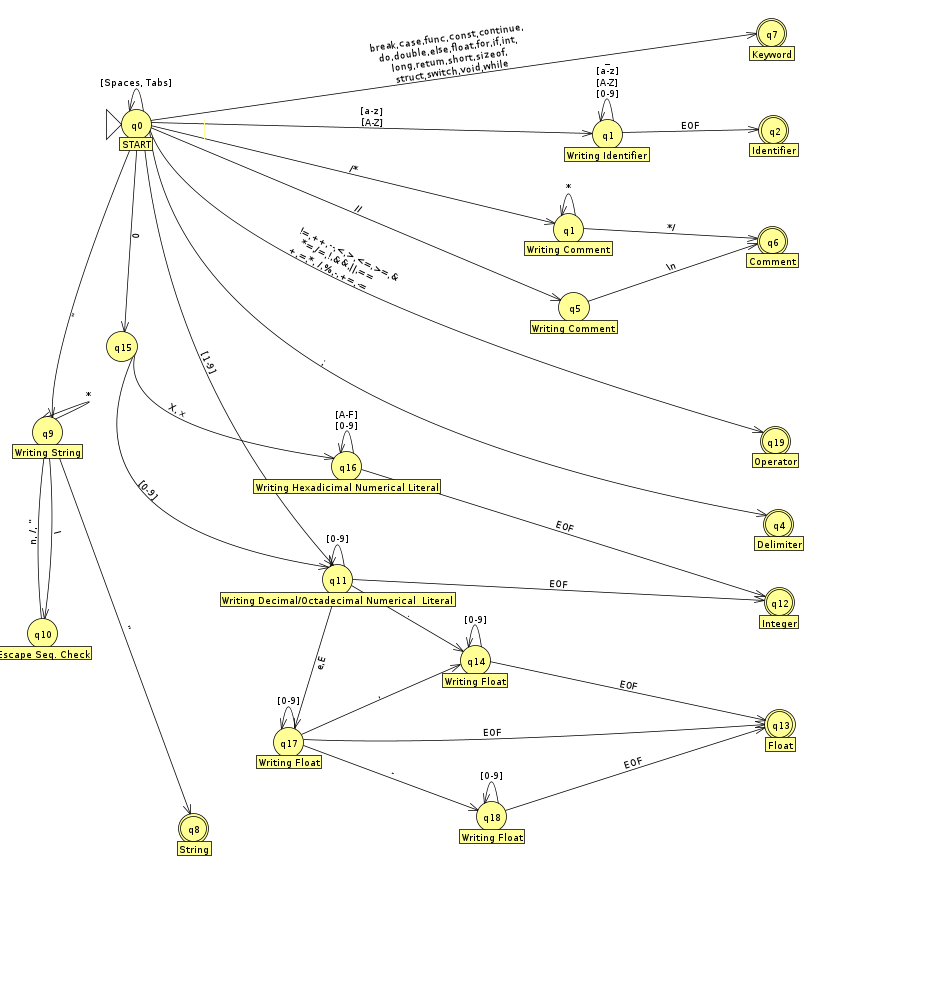
\includegraphics[scale=0.5]{automata.png}
   
\end{document}
